%追加すべき事項
% - ? Adamの詳しい説明
\appendix

\chapter{Adam}
\label{app:Adam}

Adamは勾配降下法のアルゴリズムの一つであり、\prettyref{fig:Adam}に示す手順にしたがってパラメータの更新を行う。また、Adamについては~\cite{Adam}に詳しい。

\begin{algorithm}[hb]
    \DontPrintSemicolon
    \SetKwInOut{KwHyParam}{HyperParameter}
    \SetKwInOut{KwParam}{Parameter}
    \SetKwInOut{KwObFunc}{Objective~Function~}
    \SetKwProg{Init}{Initialization}{:}{end}
    \SetKwProg{Proc}{Procedure}{:}{end}
    \BlankLine
    \BlankLine
    \KwHyParam{$\beta_1,\beta_2\in \interval[open left]{0}{1},\eta,\epsilon$}
    \KwObFunc{$f$}
    \KwParam{$\theta$}
    \BlankLine
    \Init{}{
        $t \leftarrow 0$ \tcc*{Initialize~timestep}
        $\theta \leftarrow \theta_0$ \tcc*{Initialize~Parameter}
        $m_1 \leftarrow 0$ \tcc*{Initialize~$1^{st}$~moment}
        $m_2 \leftarrow 0$ \tcc*{Initialize~$2^{nd}$~moment}
    }
    \BlankLine
    \Proc{}{
        \While{$\theta$ not converged}{
            $t \leftarrow t+1$ \tcc*{Update~timestep}
            $g \leftarrow \nabla _{\theta} f(\theta)$ \tcc*{Compute~gradient~of~$f(\theta)$}
            $m_1 \leftarrow \beta_1 \cdot m_1+(1-\beta_1) \cdot g$ \tcc*{Update~biased~$1^{st}$~moment}
            $m_2 \leftarrow \beta_2 \cdot m_2+(1-\beta_2) \cdot (g \odot g)$ \tcc*{Update~biased~$2^{nd}$~moment}
            $\hat{m_1} \leftarrow m_1/(1-\beta_1^t)$ \tcc*{Compute~bias-corrected~$1^{st}$~moment}
            $\hat{m_2} \leftarrow m_2/(1-\beta_2^t)$ \tcc*{Compute~bias-corrected~$2^{nd}$~moment}
            $\theta \leftarrow \theta - \eta \cdot \hat{m_1}/(\sqrt{\hat{m_2}}+\epsilon)$ \tcc*{Update~Parameter}
        }
        \Return{$\theta$}
    }
    \BlankLine
\caption[]{Adamの疑似コード}
\label{fig:Adam}
\end{algorithm}

\chapter{学習時のパラメータ}
\label{app:params}

\prettyref{tab:params1}に提案モデルの学習時のパラメータを示し、\prettyref{tab:params2}にAdamのハイパーパラメータを示す。

\begin{table}[h]
\centering
\begin{minipage}[b]{0.49\columnwidth}
    \centering
        \begin{tabular}{lr}\toprule
            パラメータ & 値 \\ \midrule
            バッチサイズ & 1 \\ 
            エポック数 & 1000 \\ \bottomrule
        \end{tabular}
    \caption{}
    \label{tab:params1}
\end{minipage}
\begin{minipage}[b]{0.49\columnwidth}
    \centering
        \begin{tabular}{lr}\toprule
            パラメータ & 値 \\ \midrule
            $\beta_1$ & 0.5 \\
            $\beta_2$ & 0.999 \\
            $\eta$ & 0.0002 \\ 
            $\epsilon$ & $10^{-8}$ \\ \bottomrule
        \end{tabular}
    \caption{}
    \label{tab:params2}
\end{minipage}
\end{table}

\chapter{データセットの分割}
\label{app:split}

22音ずつの4つのサブセットにデータセットを分割した~(\prettyref{fig:data_div})~。また、データセットの4分割は、88音をシャッフルして配列に格納した後に22音ずつ順に選ぶことで行った。

\begin{figure}[h]
\centering
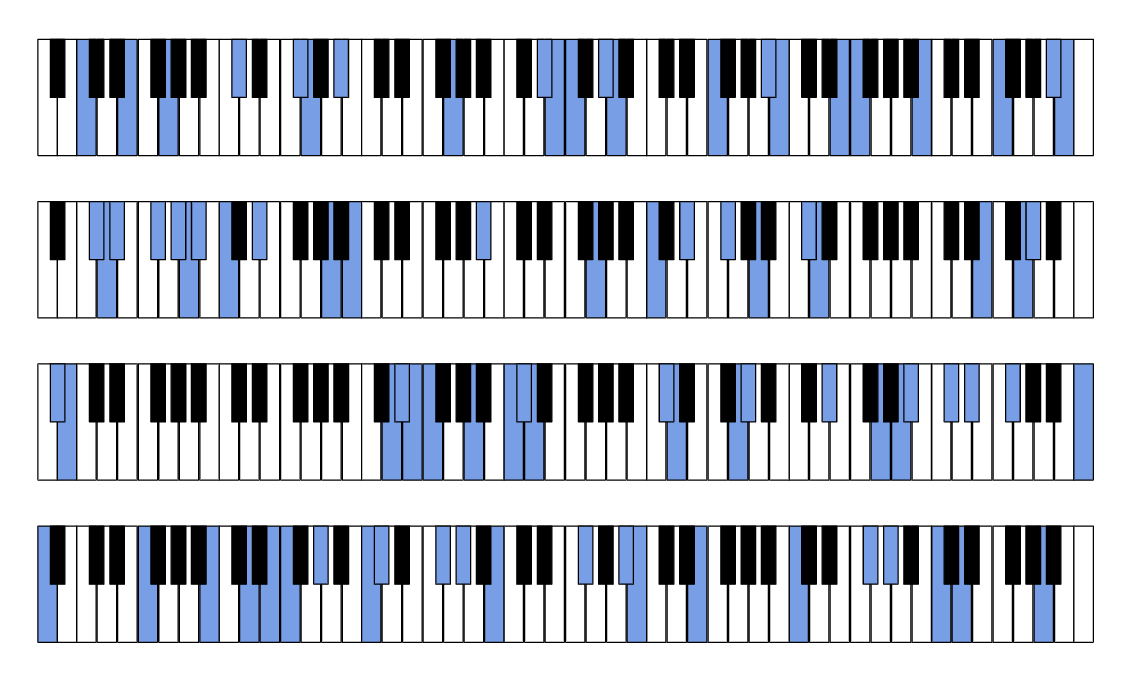
\includegraphics[width=\columnwidth]{figure/data_div.png}
\caption[]{データセットのサブセット}
\label{fig:data_div}
\end{figure}

\chapter{実験結果}
\label{app:result}

\prettyref{sec:result}に載せることのできなかった波形の図を本章に載せる。また、波形の記載方法は\prettyref{sec:result}と同様であるが、簡略化のため、キャプションには音階名のみ載せている。

\section{提案モデルの表現力の評価実験}

\appfig{figure/88_88/}{a0.png}{A0}{a0s.png}{A0$\sharp$}{b0.png}{B0}{c1.png}{C1}
\appfig{figure/88_88/}{c1s.png}{C1$\sharp$}{d1.png}{D1}{d1s.png}{D1$\sharp$}{e1.png}{E1}
\appfig{figure/88_88/}{f1.png}{F1}{f1s.png}{F1$\sharp$}{g1.png}{G1}{g1s.png}{G1$\sharp$}
\appfig{figure/88_88/}{a1.png}{A1}{a1s.png}{A1$\sharp$}{b1.png}{B1}{c2.png}{C2}
\appfig{figure/88_88/}{c2s.png}{C2$\sharp$}{d2.png}{D2}{d2s.png}{D2$\sharp$}{e2.png}{E2}
\appfig{figure/88_88/}{f2.png}{F2}{f2s.png}{F2$\sharp$}{g2.png}{G2}{g2s.png}{G2$\sharp$}
\appfig{figure/88_88/}{a2.png}{A2}{a2s.png}{A2$\sharp$}{b2.png}{B2}{c3.png}{C3}
\appfig{figure/88_88/}{c3s.png}{C3$\sharp$}{d3.png}{D3}{d3s.png}{D3$\sharp$}{e3.png}{E3}
\appfig{figure/88_88/}{f3.png}{F3}{f3s.png}{F3$\sharp$}{g3.png}{G3}{g3s.png}{G3$\sharp$}
\appfig{figure/88_88/}{a3.png}{A3}{a3s.png}{A3$\sharp$}{b3.png}{B3}{c4.png}{C4}
\appfig{figure/88_88/}{c4s.png}{C4$\sharp$}{d4.png}{D4}{d4s.png}{D4$\sharp$}{e4.png}{E4}
\appfig{figure/88_88/}{f4.png}{F4}{f4s.png}{F4$\sharp$}{g4.png}{G4}{g4s.png}{G4$\sharp$}
\appfig{figure/88_88/}{a4.png}{A4}{a4s.png}{A4$\sharp$}{b4.png}{B4}{c5.png}{C5}
\appfig{figure/88_88/}{c5s.png}{C5$\sharp$}{d5.png}{D5}{d5s.png}{D5$\sharp$}{e5.png}{E5}
\appfig{figure/88_88/}{f5.png}{F5}{f5s.png}{F5$\sharp$}{g5.png}{G5}{g5s.png}{G5$\sharp$}
\appfig{figure/88_88/}{a5.png}{A5}{a5s.png}{A5$\sharp$}{b5.png}{B5}{c6.png}{C6}
\appfig{figure/88_88/}{c6s.png}{C6$\sharp$}{d6.png}{D6}{d6s.png}{D6$\sharp$}{e6.png}{E6}
\appfig{figure/88_88/}{f6.png}{F6}{f6s.png}{F6$\sharp$}{g6.png}{G6}{g6s.png}{G6$\sharp$}
\appfig{figure/88_88/}{a6.png}{A6}{a6s.png}{A6$\sharp$}{b6.png}{B6}{c7.png}{C7}
\appfig{figure/88_88/}{c7s.png}{C7$\sharp$}{d7.png}{D7}{d7s.png}{D7$\sharp$}{e7.png}{E7}
\appfig{figure/88_88/}{f7.png}{F7}{f7s.png}{F7$\sharp$}{g7.png}{G7}{g6s.png}{G7$\sharp$}
\appfig{figure/88_88/}{a7.png}{A7}{a7s.png}{A7$\sharp$}{b7.png}{B7}{c8.png}{C8}

\clearpage

\section{提案モデルの汎化能力の評価実験}

\appfig{figure/66_22/}{a0.png}{A0}{a0s.png}{A0$\sharp$}{b0.png}{B0}{c1.png}{C1}
\appfig{figure/66_22/}{c1s.png}{C1$\sharp$}{d1.png}{D1}{d1s.png}{D1$\sharp$}{e1.png}{E1}
\appfig{figure/66_22/}{f1.png}{F1}{f1s.png}{F1$\sharp$}{g1.png}{G1}{g1s.png}{G1$\sharp$}
\appfig{figure/66_22/}{a1.png}{A1}{a1s.png}{A1$\sharp$}{b1.png}{B1}{c2.png}{C2}
\appfig{figure/66_22/}{c2s.png}{C2$\sharp$}{d2.png}{D2}{d2s.png}{D2$\sharp$}{e2.png}{E2}
\appfig{figure/66_22/}{f2.png}{F2}{f2s.png}{F2$\sharp$}{g2.png}{G2}{g2s.png}{G2$\sharp$}
\appfig{figure/66_22/}{a2.png}{A2}{a2s.png}{A2$\sharp$}{b2.png}{B2}{c3.png}{C3}
\appfig{figure/66_22/}{c3s.png}{C3$\sharp$}{d3.png}{D3}{d3s.png}{D3$\sharp$}{e3.png}{E3}
\appfig{figure/66_22/}{f3.png}{F3}{f3s.png}{F3$\sharp$}{g3.png}{G3}{g3s.png}{G3$\sharp$}
\appfig{figure/66_22/}{a3.png}{A3}{a3s.png}{A3$\sharp$}{b3.png}{B3}{c4.png}{C4}
\appfig{figure/66_22/}{c4s.png}{C4$\sharp$}{d4.png}{D4}{d4s.png}{D4$\sharp$}{e4.png}{E4}
\appfig{figure/66_22/}{f4.png}{F4}{f4s.png}{F4$\sharp$}{g4.png}{G4}{g4s.png}{G4$\sharp$}
\appfig{figure/66_22/}{a4.png}{A4}{a4s.png}{A4$\sharp$}{b4.png}{B4}{c5.png}{C5}
\appfig{figure/66_22/}{c5s.png}{C5$\sharp$}{d5.png}{D5}{d5s.png}{D5$\sharp$}{e5.png}{E5}
\appfig{figure/66_22/}{f5.png}{F5}{f5s.png}{F5$\sharp$}{g5.png}{G5}{g5s.png}{G5$\sharp$}
\appfig{figure/66_22/}{a5.png}{A5}{a5s.png}{A5$\sharp$}{b5.png}{B5}{c6.png}{C6}
\appfig{figure/66_22/}{c6s.png}{C6$\sharp$}{d6.png}{D6}{d6s.png}{D6$\sharp$}{e6.png}{E6}
\appfig{figure/66_22/}{f6.png}{F6}{f6s.png}{F6$\sharp$}{g6.png}{G6}{g6s.png}{G6$\sharp$}
\appfig{figure/66_22/}{a6.png}{A6}{a6s.png}{A6$\sharp$}{b6.png}{B6}{c7.png}{C7}
\appfig{figure/66_22/}{c7s.png}{C7$\sharp$}{d7.png}{D7}{d7s.png}{D7$\sharp$}{e7.png}{E7}
\appfig{figure/66_22/}{f7.png}{F7}{f7s.png}{F7$\sharp$}{g7.png}{G7}{g6s.png}{G7$\sharp$}
\appfig{figure/66_22/}{a7.png}{A7}{a7s.png}{A7$\sharp$}{b7.png}{B7}{c8.png}{C8}
